\PassOptionsToPackage{svgnames,dvipsnames}{xcolor}

\documentclass[12pt]{cmuthesis}
% \usepackage[left=1.5in, right=1in]{geometry} % Custom margins
% \setlength{\oddsidemargin}{1.75in}  % Left margin for odd pages
% \usepackage[showframe, left=1.5in, right=1in]{geometry}


\usepackage[Lenny]{fncychap}
\ChNameVar{\Large}

\input{sections/packages}
\input{sections/macros}

\usepgfplotslibrary{external}
\tikzexternalize

\draftstamp{\today}{DRAFT}

\begin {document}
\frontmatter

\pagestyle{empty}

\title{{\bf The Expanse: Advnaces in Design, Optimization, and Simulation\\ of Pantographic Structures}}
\author{Mitchell Bennett Fogelson}
\date{June 2025}
\Year{2025}
\trnumber{CMU-ME-00-00}

\committee{
\begin{tabular}{c}
Zachary Manchester, Chair\\
Jonathan Cagan  \\
Minchen Li  \\
Jeffrey I. Lipton (\textit{Northeastern University}) \\
\end{tabular}
}

\support{}
\disclaimer{}

\keywords{linkage design, co-design, differentiable physics, generative ai, state-estimation, deployable structures, space deployables}

\maketitle

\begin{dedication}
  TODO
\end{dedication}

\begin{abstract}
The capabilities of our robotic systems are mostly being thought as limitations of control algorithms, compute power, and complex models. Robot designs have all but converged on the serial chain solutions, which are easy to design, optimize fixed continuous parameters and conform to the existing simulation frameworks. However these solutions are failing to understand the influence and trade-off between more complex designs whose geometry, composition, and compliance enable behaviors without the need for complex control, models or compute. In the aerospace community these designs have been essential to achieve the successful missions of systems like James Webb and many more. However, the systems require lots of physical testing and analysis to ensure success. In this work we imporve the capabilities of pantographic designs, reduce the design burden with new optimization methods, and introduce a differentiable simulation that supports these design for analysis and control. This thesis advances the capabilies of mechanical systems for robotic and aerospace solutions for future missions and goals. 
\end{abstract}

\newgeometry{left=0.5in,right=0.5in,top=1in,bottom=1.4in}
\begin{acknowledgments}
TODO 
\end{acknowledgments}
\restoregeometry

\pagestyle{plain}

\tableofcontents
\addtocontents{toc}{\vspace*{-2cm}}
\listoffigures
\addtocontents{lof}{\vspace*{-2cm}}
\listoftables
\listofalgorithms

\mainmatter

\chapter{Introduction}

This dissertation introduces ... TODO \cite{fogelson2024herds}

In the period between ... TODO 

% % commented out until I actually do it 
% In Chapter \ref{sec:herds} 

% Chapter \ref{sec:gcpholo}

% Chapter \ref{sec:capo}

% Chapter \ref{sec:cckdojo}

% Chapter \ref{sec:cloth}

% Chapter \ref{sec:zerog}

% With these works this dissertation is able to ...


\newpage
\section{Summary of publications}
\newcommand{\fcite}[1]{
  \begin{leftbar}
  \begin{quote}%
    \citep{#1} \fullcite{#1}
  \end{quote}
  \end{leftbar}}

% \noindent The content of \cref{sec:herds} appears in:
% \fcite{tracy2024}
% \vspace{5mm}

% \noindent The content of \cref{sec:gcpholo} appears in:
% \fcite{tracy2022c}
% \vspace{5mm}

% \noindent The content of \cref{sec:capo} appears in:
% \fcite{tracy2023}
% \vspace{5mm}

% \noindent The content of \cref{sec:cckdojo} appears in:
% \fcite{tracy2022a}
% \vspace{5mm}

% \noindent The content of \cref{sec:cloth} appears in:
% \fcite{tracy2023b}
% \vspace{5mm}

% \noindent The content of \cref{sec:zerog} appears in:
% \fcite{tracy2023d}
% \vspace{5mm}




%%% Local Variables:
%%% coding: utf-8
%%% mode: latex
%%% TeX-engine: xetex
%%% TeX-master: "../thesis"
%%% End:
\chapter{Background}
\label{sec:background}
This chapter provides a thorough description of ... TODO


\section{Pantographic Structures}

\section{Reinforcement Learning}

\section{Mixed Integer Optimization}

\section{Differentiable Simulation}

\section{State Estimation}

\section{System Identification}


%%% Local Variables:
%%% coding: utf-8
%%% mode: latex
%%% TeX-engine: xetex
%%% TeX-master: "../thesis"
%%% End:


\graphicspath{{sections/01_HERDS_Composition/}}

\chapter{Non-Planar Hierarchical Composition of Extending Metamaterials for Deployable Load-Bearing Structures}\label{sec:herds}
Structures and materials with geometric hierarchy exhibit enhanced strength-to-weight ratio. In volume-constrained scenarios, such as packing payloads into a rocket fairing, deployable structures enable the efficient transport of load-bearing forms. When optimizing the strength-to-packing efficiency of payloads, this work shows that non-planar hierarchical compositions {of deployable structures} can dramatically improve performance. To this end, the paper describes {a new pantographic design,} the Pop-Up Extending Truss (PET), which uses the composition of scissor elements to enable out of plane reorientation, enhancing the bending stiffness by over 100\% compared to other translational scissor variants with equal mass and linear packing. Additionally, by composing multiple PET structures in a Kresling pattern we show this new structure - which is refered to as HERDS (Hierarchical Extending and Reorienting Deployable Structures) - is capable of supporting 10x higher bending, compressive, torsional, and tensile stiffness at 25-200x extension ratios compared to non-hierarchical {deployable} structures when designs are constrained by initial volume. A physical HERDS prototype achieved a 50x extension ratio and supported compressive and bending loading. Practical applications for this new {class of} deployable structures include large space structures, deployable infrastructure, and compact medical devices.

\begin{figure}
\centering
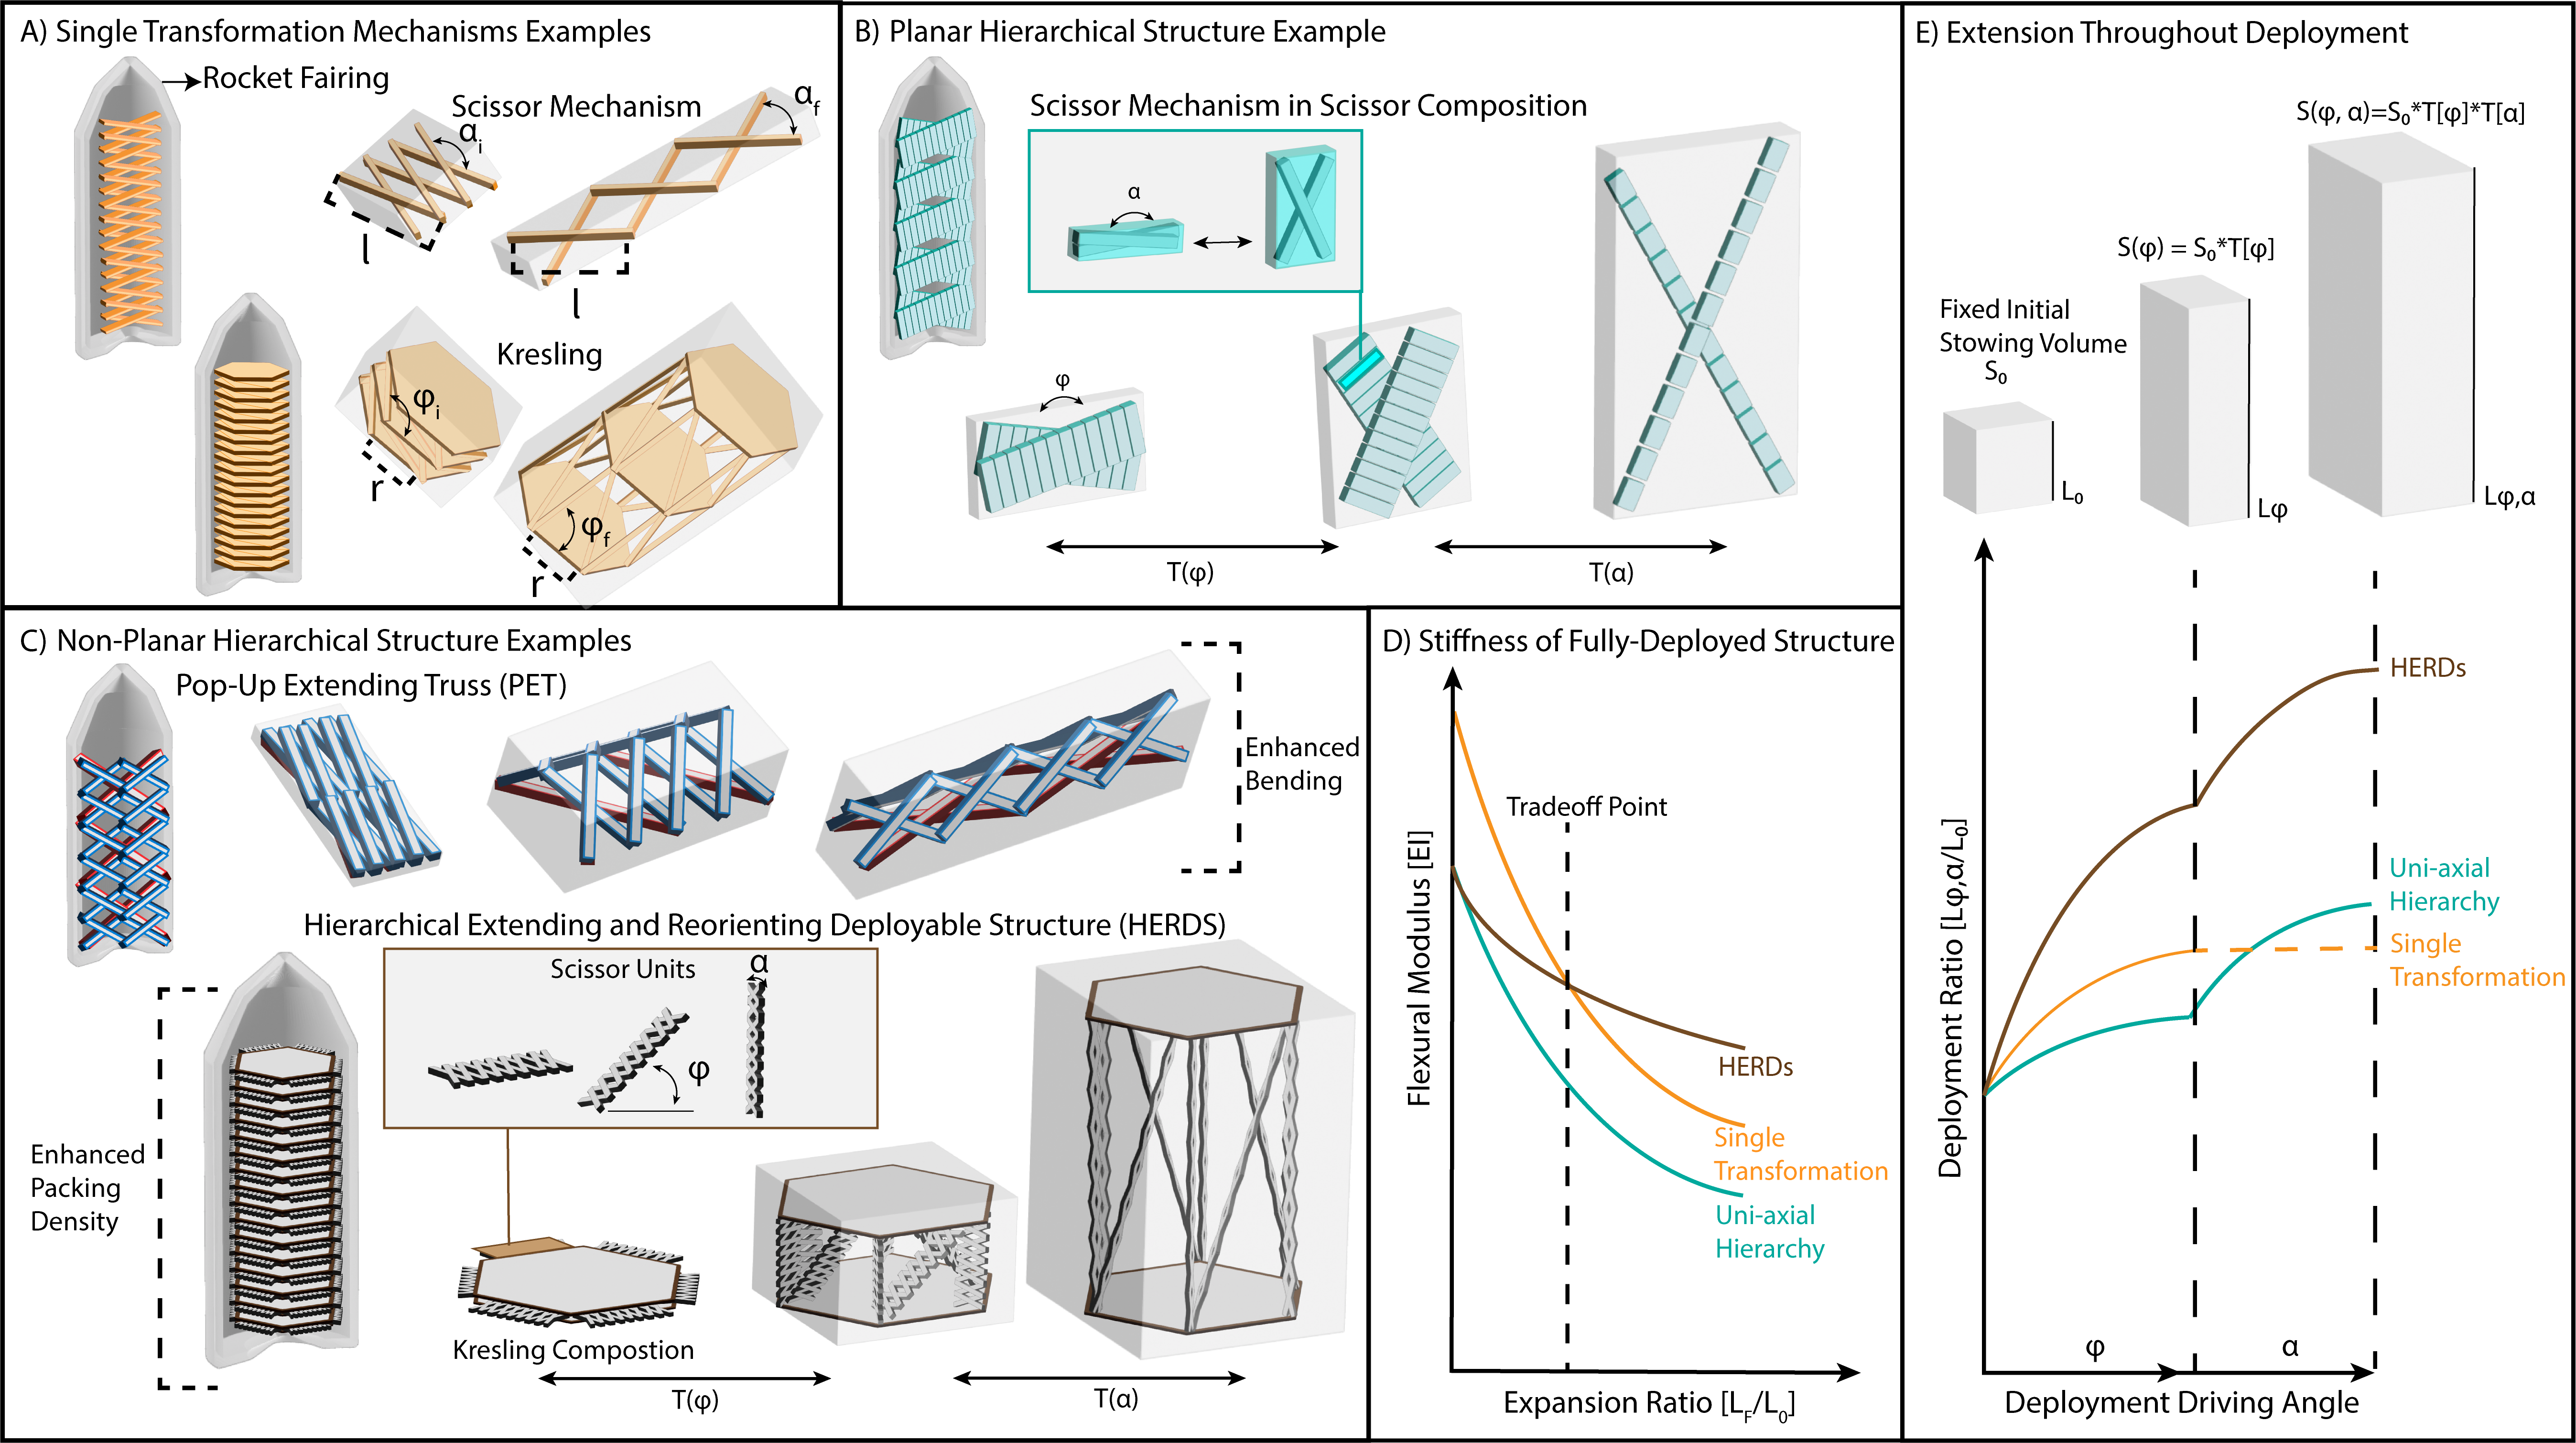
\includegraphics[width=\textwidth]{Figures/Rebuttal/figure1_orientation_change_rebuttal_05_09.png}
\centering
\caption{This figure illustrates various mechanical design concepts for structures that can extend: \textbf{A) Single Transformation Mechanisms:} shows a scissor mechanism representing a structure that leverages folding and a Kresling origami structure that leverages wrapping transformation.~\textbf{B) Hierarchical Deployment (Same Axis Transformation):} demonstrates a two-step transformation along the same axis showing a large area change, but not a useful hierarchy for extension applications.~\textbf{C) Hierarchical Deployment (Multi-Axis Transformation):} depicts a multi-axis transformation where the structure goes through a hierarchical expansion that supports extension through both deployment transformations.~\textbf{D) Graph of Bending Stiffness vs. Expansion Ratio:} shows the relationship between bending stiffness and the expansion ratio, highlighting a trade-off point. It compares different design strategies: HERDs (hierarchical expansion of reorienting designs), single transformation mechanisms, and uni-axial hierarchy.~\textbf{E) Expansion Given Constant Beam Width:} visualizes the volume expansion \(V0\) from an initial compact state $L0$ through the transformations $T(a)$ and $T(b)$ to reach a final expanded state $L(a, B)$, while maintaining a constant beam width.}\label{fig:expansion}
\end{figure}

\section{Introduction}\label{sec:herds:introduction}
{Engineers continue to push the boundaries of large-scale space structures to extend the capabilities outside of earth. One such example of this is the James Webb Space Telescope, with its sun shield spanning over 10 tennis courts, enabling the capture of unprecedented images of the universe. Previous work by the authors proposed a preliminary evaluation of a kilometer-scale space structure from a single rocket launch to support artificial gravity~\cite{fogelson2024herds}. A kilometer-scale design is 50x longer than the JWST and 10x longer than the current ISS. The design of such a structure must optimize strength-to-packaging efficiency to achieve this in a single launch with existing space vehicles. Alternative approaches aim to replicate Earth-based construction methods by transporting raw materials and assembling structures in space~\cite{xue_review_2021}. However, this requires advanced coordinated robotic systems, which is an area of ongoing research. More commonly, as seen with JWST, a collapsible structure is prefabricated on Earth and compactly stowed for a launch with no in-space assembly required. This work builds on the previous study by the authors \cite{fogelson2024herds} by performing a more extensive design sweep of the non-planar hierarchical deployable mechanism and its subcomponents, offering a deeper analysis of design parameters, trade-offs, and metamaterial behavior in PET and HERDS structures.}

The aerospace and architecture industry has led advances in single-transforming load-bearing mechanisms as described in \cite{doi:10.1177/0266351117711290}. The aerospace community, constrained by rocket fairing size has demonstrated many examples of booms~\cite{chu_design_2014,fernandez_advanced_2017,noauthor_lightweight_2004,you_self-locking_2006,yang_wrapping_2019,yang_novel_2022,wang_blossoming_2020,shore_effects_2021,salazar_experimental_2021} and masts~\cite{brown_deployable_2011,harrison_nuclear_2013,li_deployment_2016,nagaraj_kinematics_2009, tibert_deployable_nodate,you_cable-stiffened_1996,yu_nonlinear_2021}. Although past successes have demonstrated the viability of these approaches, continued innovation remains crucial for future missions. 

{In the literature, many extending space structures exist, which have been segmented by Wang et al. \cite{WANG2024112557}, in a review paper on deployable space structures, into inflatable, elastic, and pantographic solutions. All of these structure types have a place in the space infrastructure landscape, and no one solution is a silver bullet for current and future deployable structure problems.} 

{Inflatable deployable mechanisms offer several advantages over rigid structures, particularly in terms of weight reduction and high packaging efficiency. In the review paper by Wang et al. \cite{WANG2024112557}, they include the following successful examples of inflatable deployable structures include the inflatable antenna used in the Echo I mission \cite{grahne2001deployment}, the antenna deployed on the STS-123 Space Shuttle Endeavor \cite{cooper2009rigidizable}, the inflatable radar (SAR) for Earth-sensing missions \cite{lou2000development}, and the inflatable solar arrays used on the Mars Rover \cite{cadogan1999inflatable}. However, several technical challenges remain, including optimizing packing strategies \cite{schenk2014review}, understanding inflation dynamics \cite{cui2012overview}, and developing accurate models \cite{dollah2017inflatable}. For kilometer-scale space structures intended for artificial gravity, inflatable systems are less suitable due to their susceptibility to micrometeoroid impacts and vulnerability to global buckling failure.}

{The use of thin-walled elastic members is touted for their high strength-to-weight properties and simple construction~\cite{fernandez_advanced_2017,yang_wrapping_2019,salazar_experimental_2021}. Variations of such structures display extension ratios exceeding 300x, but rely on material elasticity to deploy and maintain their structure~\cite{salazar_experimental_2021}. {Practical examples of these systems are the iROSA structures on the ISS \cite{schwanbeck2019advanced} and DaGHR antenna \cite{kelly2016scalable}. Although these structures offer advantages in self-deployment, the release of stored strain energy is often unpredictable, difficult to control, and highly dynamic. This can lead to unwanted vibrations and potential secondary damage. Thin-walled composite structures also suffer from low impact resistance, presenting durability challenges in space environments~\cite{noauthor_lightweight_2004}. Additionally, these structures face scaling limitations due to the significant elastic energy stored during deployment and their lower structural rigidity compared to conventional truss systems, making them less viable for kilometer-scale applications in microgravity.}} 

{Deployable truss structures, also known as pantographic structures, offer design versatility, allowing for customization and adaptation to various configurations based on specific deployment requirements. Compared to telescopic structures, they provide a higher spatial packaging efficiency and reduced weight. However, their design and deployment mechanisms are inherently complex and often require a large number of parts. In addition, Pantagraphic structures are limited by the aspect ratio or material thickness to achieve higher extension ratios. For a scissor-based mechanism, that means that the individual truss elements become very long and thin, leading to the possibility of local buckling. In the review paper by Wang et al. \cite{WANG2024112557}, they highlight the following deployable truss structures have been implemented in various applications, including extension masts ~\cite{kitamura1990development, tibert_deployable_nodate,perez-valcarcel_new_2021,kim_deployable_2021,puig_review_2010}, extension arms \cite{choi2019design}, flexible solar array paddles \cite{kojima1996development}, and telescopic masts for NASA’s Shuttle Radar Topography Mission \cite{umland2012STRM}. Parallel deployable truss structures have been utilized in planar solar arrays, such as those on the Chinese Dongfanghong (DFH)-4 \cite{yuanyuan2022parameter} and DFH-5 \cite{ma2022recent} satellites, the Spacebus Earth communication satellite \cite{tian2021research}, and the Shijian 20 satellite \cite{cui2020orbit}. Another common application is for parabolic antennas, including those on the ETS-VIII \cite{meguro2009orbit} and Environment-1C \cite{shi2014design} satellites, as well as in MegaFlex solar arrays \cite{zhou2015development}. These applications benefit from pantographic structures, which are inherently free of strain energy, material-agnostic, and scalable, making them well-suited for large deployable systems. To the authors' knowledge, no kilometer-scale deployable truss structure has been deployed.} 

\begin{table}[ht]
    \centering
    \begin{tabular}{|c|c|c|c|c|} \hline
        & Inflatables & Elastic & Pantographic & \parbox[c]{3.5cm}{\centering \textbf{Non-Planar Hierarchical}\\ \textbf{Pantographs (Ours)}} \\ \hline
        Controlability & $\times$ & $\times$ & $\checkmark$ & $\boldsymbol\checkmark$ \\ \hline
        Retractability & $\times$ & $\checkmark$ & $\checkmark$ & $\boldsymbol\checkmark$ \\ \hline
        Scalability & $\checkmark$ & $\times$ & $\checkmark$ & $\boldsymbol\checkmark$ \\ \hline
        Redundancy & $\times$ & $\times$ & $\checkmark$ & $\boldsymbol\checkmark$ \\ \hline
        \parbox[c]{3.5cm}{\centering {High Strength to}\\ {Packing Ratio}} & $\checkmark$ & $\checkmark$ & $\times$ & $\boldsymbol\checkmark$ \\ \hline
    \end{tabular}
    
    \caption{{Comparison of deployable structure classes including Inflatables, Elastic Structures, Pantographic, and our proposed Hierarchical Pantographic Structures. Hierarchical Pantographs enhance key advantages such as retractability, scalability, and strength-to-packing ratio while maintaining the benefits of redundancy and control.}}
    \label{tab:structure_comparison}
\end{table}

{This work looks at a rocket fairing packing problem, where the structure seeks to both maximize the usable volume in the fairing in the stowed state and the linear extension in the deployed state}. At this scale, elastic deployable solutions are not feasible due to the large shear stress in the stowed state. Additionally, inflatable structures are not considered due to their limitations for bending applications. When constrained by a predetermined initial volume, Pantagraphic deployable structures must minimize material thickness to enhance packing density to achieve the necessary extension ratios. This necessity introduces an inherent compromise between the extent of extension achievable and the structure's load-bearing capacity. The geometric hierarchy in natural and architected structures improves the strength-to-density ratio for improved efficiency and performance~\cite{lakes_materials_1993,schaedler_architected_2016,bauer_nanolattices_2017, schwaiger_extreme_2019}. Biology incorporates {structural }hierarchy in their additive building processes, enabling enhanced mechanical properties~\cite{fratzl_natures_2007}. Bird bones exhibit structure on multiple length scales to match necessary loading requirements at extremely low weight~\cite{sullivan_extreme_2017}. Wood and plant stems use {structural} hierarchy to provide mechanical support against the elements~\cite{lakes_materials_1993,chen_bio-mimetic_2013}. In engineered systems, {this} hierarchy is incorporated in large structures, such as radio towers, bridges, and quite famously, the Eiffel tower~\cite{lakes_materials_1993}. {These structures are referred to as space frame structures and credited to Alexander Graham Bell in 1903~\cite{chilton_space_1999}.} With digital fabrication, hierarchical mechanical metamaterials can be tuned to exhibit extremal properties~\cite{banerjee_mechanical_2014,bauer_nanolattices_2017}. Despite the structural utility of hierarchy, the benefits of hierarchical designs of transforming and deployable structures have been muted. {We define "deployable hierarchy" as the combination of multiple transforming mechanisms arranged at different size scales, which has not been demonstrated in non-planar cases. }Planar hierarchy has demonstrated synchronized deformations and auxetic properties~\cite{xu_design_2017,gatt_hierarchical_2015}, with applications for architected area changes, but no added structural benefit over traditional extending structures (Figure \ref{fig:expansion}.B). 

Our research introduces a novel class of mechanical metamaterial structures that leverage {non-planar deployable }hierarchy to combine multiple separate deployable mechanisms at different size scales to improve the tradeoff between extension and strength-to-weight ratios with a wide range of tunable properties. This work makes the following contributions:
\begin{enumerate}
    \item We demonstrate that the non-planar {deployable }hierarchical composition of extension mechanisms enhances material packing density, improving mechanical properties at high extension ratios.
    \item By applying this framework to scissor mechanisms, we introduce the Pop-Up Extending Truss (PET) mechanism, which offers better packing density and bending properties than existing scissor-like variants.
    \item We provide an example of Hierarchical Extending and Reorienting Deployable Structures (HERDS), a {non-planar deployable hierarchical structure} that integrates the PET and Kresling mechanisms. Finite element simulations demonstrate improved mechanical properties at high extension ratios, and a prototype implementation of the structure is presented as a path toward practical applications.
\end{enumerate}


\section{Results}
\subsection{Hierarchical Composition {of Deployables} for High Extension}
\subsubsection{Composition of Linear Extension Deployables in Kresling Pattern} Through sliding, wrapping, or pivoting their material, structures can stow and expand, manipulating the pose of material members and thus volume. This work looks at structures that extend to many times their stowed length. When fully deployed, these structures can have high length-to-width ratios, making them vulnerable to bending and buckling. Therefore, the structure's extension ratio (ER) -- the ratio of the final length to the stowed length -- and flexural modulus (EI) -- a metric used to evaluate bending stiffness measured in the deployed state -- are considered to assess a structure for load-bearing applications \cite{mikulas_truss_2006}. Without a loss of generality, this work focuses on 1-DOF extending mechanisms, where a single parameter, such as the angle between the scissors, can represent the state of the structure. A structure seeking to achieve a high extension ratio must maximize the packing density by pivoting, sliding, or wrapping the subcomponents in relation to one another. The volume of a pivoting 1-DOF mechanism, such as a scissor mechanism or mechanical Kresling, described in Zhai et al. \cite{zhai_origami-inspired_2018}, can be seen in Figure \ref{fig:expansion}.A, transforms based on the rotation of the internal beams. The extension ratio for a translational scissor is expressed by:

\begin{equation}
    ER_{scissor} = \frac{l*cos(\alpha_f)}{l*cos(\alpha_i)} \approx \frac{l}{t} \quad \text{when}\quad cos(\alpha_f) \approx 1 \And n >> 1
\end{equation}
where $\alpha_i$, $\alpha_f$ are the initial and final angles of the scissor, $l$ is the link length of the scissor, $t$ is the thickness of the link, and $n$ is the number of scissor units connected together. The extension ratio of the scissor mechanism is the ratio of the cosine of the final angle between the members to the initial angle of the members. This extension ratio of a scissor can be approximated as the aspect ratio of an individual member when there are many scissor units combined. The extension ratio of a Kresling mechanism is:
\begin{equation}
    ER_{Kresling} = \frac{r\sqrt{(2*cos(\phi_f)-1)}}{r\sqrt{(2*cos(\phi_i)-1)}} \approx \frac{r}{2t} \quad \text{when}\quad \frac{t}{r} << 1
\end{equation}
where $r$ is the radius of the mechanism, $\phi_i, \phi_f$ is the angle offset between the top and bottom plates of the Kresling (twist), and $t$ is the thickness of the Kresling members. Here, the extension ratio is again a ratio of the final angle to the initial angle and can also be approximated as an aspect ratio of the kresling members, which is a function of its radius. 

This shows that the only way to achieve high extension ratios for these mechanisms is to have high aspect ratio elements that are prone to local buckling when subjected to bending loads. Similarly, for other 1-DOF mechanisms that use pivoting and sliding deployment, these designs only contain a single packing direction. This means that the magnitude of possible expansion is fully determined by the dimensions of the initial bounding volume and the thickness of the individual members making up the mechanism \ref{fig:expansion}.A. This problem is exacerbated in the practical design of deployable mechanisms when the original bounding dimensions are constrained, leading to thinner individual members, leaving designs susceptible to buckling and local deformation.

% \subsubsection{Hierarchical Non-planar Mechanisms} 
Non-planar {deployable }hierarchy can be used to increase the extension ratio while maintaining favorable member aspect ratios. One example highlighted in this paper is the composition of scissor elements and the Kresling pattern, Figure \ref{fig:expansion}.C. This new structure hierarchically extends through multiple sequential reorientations of the individual elements. This hierarchical composition enables tighter packing of the sub-mechanisms to achieve high extension ratios. The extension ratio from HERDS is approximately as follows:

\begin{equation}
    ER_{HERDS} = \frac{n*l*cos(\alpha_f)}{r\sqrt{(2*cos(\phi_i)-1)}} \approx \frac{n*l}{2t} \approx \frac{r*l}{2t^2} \quad \text{when}\quad cos(\alpha_f) \approx 1 \And \frac{t}{r} << 1
\end{equation}
where $\alpha_f$ is the angle of the scissor mechanism, $\phi_i$ is the twist angle of the Kresling, $t$ is the thickness of the scissor links, $n$ is the number of scissor units, $l$ is the length of the scissor links and $r$ is the radius of the Kresling. The hierarchical composition increases the tunable parameters to achieve high extension, including the number of scissor units, kresling deployment angle, kresling radius, and member aspect ratio. 

An important note about the proposed design from Figure \ref{fig:expansion}.C, the hierarchical composition of the mechanism transformations must occur sequentially. The Kresling transformation, $T[\phi]$, is performed first, reorienting the scissor mechanism. Then, the scissor mechanism's transformation, $T[\alpha]$, can deploy the subcomponents smoothly, increasing the system extension. These transformations are not commutable; for example, in the collapsed state, the transformation of the scissor mechanism, $T[\alpha]$, would not lead to the effective extension of the mechanism. This is not always the case when composing deployable mechanisms, as in Figure \ref{fig:expansion}.B, the transformations commute.

By manipulating the orientation of substructure stacking through {deployable }hierarchical design, we achieve high packing efficiency without increasing the component aspect ratio. This demonstrates the benefits of hierarchical deployable structures for extension ratio but does not consider the structure's stiffness yet. The stiffness of the deployed structure depends on the extended material's final deployed architecture. The next section considers various scissor structures and their effect on hierarchical design stiffness.

\subsection{Pop-Up Extending Truss: A Non-Planar Composition of Scissor Elements}
\begin{figure}
\centering
\includegraphics[width=0.9\linewidth]{Figures/Rebuttal/figure2_PET_reorientation_rebuttal.png}
\centering
\caption{This figure presents the Pop-Up Extending Truss (PET) structure, a novel scissor-like mechanism {, and a HERDS mechanism that consists of 12 PET structures in a Kresling pattern to achieve the non-planar deployable hierarchy}. \textbf{A) PET Deployment:} provides an isometric perspective of the PET, comprising three interconnected scissor elements: the blue ones are Short-Link Scissor Members (SLSM), while the red one is the Long-Link Scissor Member (LLSM). The design facilitates a compact arrangement by allowing the SLSMs to collapse onto the LLSM. Upon deployment, the SLSMs extend into a triangular truss configuration, thereby improving the structure’s resistance to bending. \textbf{B) Individual Mechanism Deployment:} showcases a solitary scissor element, depicting the PET’s top view and the pivotal state parameter alpha as it moves from a stowed to an extended state. \textbf{C) Collective Reorientation:} presents the PET’s frontal view, illustrating the transition of the SLSMs from a flat, packed condition in the stowed phase to an elevated, triangular form upon deployment. {\textbf{D) HERDS (PET + Kresling):} presents a rendering of a HERDS mechanism composed on 12 PET structures in a Kresling pattern through the deployment with the effective boundary.}}\label{fig:PET_expansion}
\end{figure}

\begin{figure}
    \centering
    \includegraphics[width=\linewidth]{Figures/Figure3 - pet testing 07-10.png}
    \centering
    \caption{This figure evaluates the performance characteristics of the Pop-Up Extending Truss (PET) against traditional solid and scissor-type beams through both theoretical and empirical analyses: \textbf{A) Flexural Modulus vs. Scissor Deployment:}  Demonstrates that as the PET deploys, maintaining a given member aspect ratio, it consistently outperforms basic scissor structures in flexural modulus. However, these scissor variants do not achieve a higher utility than a solid beam within the depicted extension ratio range, showing a $42.9\%$ reduction in normalized flexural modulus for the solid beam. \textbf{B) Flexural Modulus vs. Link Aspect Ratio:} Illustrates the threshold at which the PET's short-link scissor member's aspect ratio surpasses the utility of a conventional solid beam, indicating a $71\%$ increase in normalized flexural modulus.\@\textbf{C) Physical Testing:} Depicts the physical test units used in an Instron machine, which were instrumental in validating and calibrating the simulation models developed in ANSYS.\@\textbf{D) Physical Testing vs. Simulation:} Confirms the alignment between the beam model approximations and the physical testing results, showing a close correlation between the observed physical and the simulated flexural stress across a range of flexural strains for the PET, short-link scissor and long-link scissor beams.}~\label{fig:flex_comp}
\end{figure}
A translational scissor mechanism has a low flexural modulus when fully deployed, making it susceptible to bending failures. Using a translational scissor mechanism as the substructure for the HERDS leads to a major limitation of the overall mechanical stiffness. Through finite element analysis, the flexural modulus (bending stiffness) of the scissor mechanism is shown to be less than that of a solid beam with the same cross-sectional area, as seen in Figure \ref{fig:flex_comp}.A. While the hierarchical composition of a scissor and Kresling mechanism provides extension benefits, the poor bending stiffness limits the usefulness of the hierarchical design. 

\subsection{Improved Bending Stiffness}
By applying a non-planar composition of scissor mechanisms, we developed a novel deployable structure known as the Pop-Up Extending Truss (PET), first described by Fogelson et al. in \cite{fogelson2024herds}. {The PET consists of three scissor mechanisms: two short-link translational units and one long-link translational unit with a polar offset. This offset enables out-of-plane motion during deployment, resulting in multi-axis reorientation of the substructures.} This unique composition allows the structure to simultaneously extend and expand, forming a triangular truss configuration (Figure \ref{fig:PET_expansion}). {The PET differs from other triangular scissor mechanisms, such as \cite{you_cable-stiffened_1996}, which retain a triangular void in the center when collapsed. In contrast, the PET structure flat-packs, significantly improving packaging density and making it well-suited for integration into a non-planar deployable hierarchy following a Kresling pattern.}

{In the stowed state, the long scissor unit occupies the width of the two smaller units, enabling flat packing. As the PET deploys, the width of the long scissors changes at a different rate than that of the short scissors, which forces an out-of-plane reorientation and results in the formation of a triangular truss.} This geometric transformation increases the structure’s minimum bending moment of inertia, thereby enhancing its resistance to bending and buckling.

For this analysis, all structures were modeled using beam-based finite element methods (FEM) to evaluate comparative structural performance. The material type and Young’s modulus ($E$) were held constant, so differences in stiffness are primarily due to changes in the bending moment of inertia, $I_x = \int_A y^2 dA$ or $I_y = \int_A x^2 dA$. In idealized systems, placing structural mass further from the centroid increases bending and buckling resistance. {However, in truss and lattice-based structures, both local and global deformation modes must be considered as the aspect ratios and densities of constituent beams change.} {To evaluate performance, we conducted a simulated cantilever beam test across various extending topologies—independent scissor mechanisms, the PET, and a solid reference beam with equivalent bundled cross-sectional area—under the weakest configuration: in-plane bending with a fixed displacement.} Flexural modulus was estimated using:
\begin{equation}
    EI = \frac{FL^3}{3d}
\end{equation}
where $F$ is the reaction force, $L$ is the effective length of the mechanism, and $d$ is the tip displacement.

{Figure \ref{fig:flex_comp}.A shows that as the PET extends, its effective flexural modulus increases at a greater rate than either of the short- or long-link scissor mechanisms alone, with a maximum observed improvement of $68\%$ over a solid beam with equivalent bundled cross-sectional area. We additionally compare the PET to independent short- and long-link scissor mechanisms adjusted to have equal mass by increasing their cross-sectional area. The PET, when built from square-cross-section beams, achieves a $50\%$ stowing advantage over an equivalent-mass scissor mechanism with rectangular cross-section. Structurally, the PET demonstrates a $111\%$ bending stiffness improvement over the long-link scissor and a $115\%$ improvement over the short-link scissor.} 

{To validate the accuracy of the beam model approximation used in the FEA simulation, we conducted physical tests using an Instron machine, as shown in Figure \ref{fig:flex_comp}.C. The correlation between the experimental results and the simulated structures is illustrated in Figure \ref{fig:flex_comp}.D. Additional information about the Sim2Real validation and parameters can be found in SM Section 5.}

\subsubsection{Scaling Effects of PETS} To understand the PET design space tradeoffs, Figure \ref{fig:flex_comp}.B compares the PET flexural modulus of various member aspect ratios to a square cross-sectional beam of equal area. At low aspect ratios (shorter/thicker members), the mass of the PET remained close to the centroid, offering no significant moment of inertia benefit while simultaneously having sparse connectivity. As a result, the solid beam outperformed the PET. As PET member aspect ratios increased, the material was distributed farther from the centroid, causing the effective bending moment of inertia to increase. When the minimal aspect ratio of the PET surpassed 9.28, we saw improved flexural modulus results compared to those of the solid beam. As the PET member aspect ratio continued to increase, local bending of the slender beams became the dominant deformation mode, and the PET flexural modulus asymptotically approached 71\% improvement over the solid beam. 

The PET's aspect ratio directly correlates to the extension ratio (ER) and bending stiffness. By mass, hierarchical deployable structures with PETs as subcomponents only become structurally beneficial when the PET supports higher extension ratios. Many applications for deployable structures are volume rather than mass-constrained, making packing density an important consideration along with relative flexural modulus. The bespoke design enables the members to attain a stowage density of $50\%$ greater by reducing the height in the direction orthogonal to expansion, as opposed to a scissor mechanism with the same extension ratio and mass. This stowing benefit does not directly boost the ER of the PET, but within HERDS, the increased stowed density aligns with the extension axis.

\subsection{Design Tradeoffs of {Non-Planar Hierarchical Deployable}  Mechanisms}
{In this section, we revisit the volume-constrained design problem introduced in Section \ref{sec:herds:introduction}, focusing on the creation of kilometer-scale deployable structures from a single launch, Figure \ref{fig:enter-label}.A. We conduct a global design space sweep comparing the performance of the proposed non-planar hierarchical mechanism (HERDS) with its constituent substructures: the PET and Kresling (KRES) mechanisms. To systematically evaluate these structures, we generated over 2,300 designs—approximately 500 HERDS, 1,000 PETs, and 800 KRES—by sweeping key geometric parameters including member thickness and deployment angle, Figure \ref{fig:enter-label}.B. These parameters were selected for their direct impact on stowed and deployed height, allowing us to sample designs across a wide range of extension ratios (5x–200x).}

{All designs were simulated using Finite Element Analysis (FEA) in ANSYS\textregistered APDL\cite{ansys_inc_ansys_nodate}, accessed through its Python API~\cite{alexander_kaszynski_2020_4009467}. The structures were modeled using BEAM188 elements with fixed joints (excluding joint mass) and subjected to bending, tension, compression, and torsional loading. For bending, compression, and tension simulations, we applied a displacement equal to $1\%$ of the final structure length, while torsional analysis used a fixed angular displacement of 3.6°. A full description of model assumptions, material properties, boundary conditions, and solver settings is included in SM Section 5.3, 5.4, 6, SM Figure 8-9, and SM Table 2-3.}

{To contextualize performance across varying sizes and topologies, all results were normalized using the average performance of the HERDS designs. This allows for a clear comparison of stiffness trends across different structures and extension ratios. Only designs with extension ratios greater than or equal to 77x meet the kilometer-scale deployment target, however, we report results across the entire sampled range (5x–200x) to identify the threshold at which HERDS surpasses its substructures. Data corresponding to extension ratios below 77x is shaded in grey in Figures \ref{fig:enter-label}.C–F.}

{The results of this study reveal that hierarchical structures (HERDS) consistently outperform PET and KRES mechanisms in all loading conditions—bending, compression, tension, and torsion—once the extension ratio exceeds approximately 25x. Figure \ref{fig:enter-label}.C–F plots normalized stiffness as a function of extension ratio for each loading mode. As expected, stiffness generally decreases with increasing extension ratio across all structures. However, the rate of decline varies significantly.}

{KRES designs exhibit relatively high stiffness in bending, compression, and tension at low extension ratios but degrade sharply beyond 25x, often failing to converge due to local buckling instabilities. Furthermore, KRES designs perform the worst under torsional loading across all extension ratios, likely due to their unidirectional rotational compliance.}

{PET designs, on the other hand, demonstrate excellent deployment stability up to a 200x extension ratio without local buckling, particularly excelling in torsional stiffness. However, PETs show weaker bending, compression, and tension stiffness at low-to-moderate extension ratios when compared to KRES. This performance gap is likely due to the underutilization of available fairing volume, as PETs only occupy a small portion of the 5-meter diameter constraint.}

{HERDS structures strike a compelling balance between deployability and structural integrity. Beyond 25x extension, they consistently outperform both PET and KRES structures in all loading conditions. Importantly, these trends persist even after normalizing by mass, as shown in Figure SM 9 in the supplementary materials. However, we note that hierarchy is not always beneficial: below 25x extension, simpler substructures may offer better performance. Still, across the full design sweep, hierarchical composition reduces stiffness degradation at high extension ratios, validating the mechanical advantages of the HERDS approach.}

{To further explore these findings, we fabricated and tested a physical HERDS prototype, as described in the following section, to assess practical implementation and deployment reliability.}

\begin{figure}
    \centering
    \includegraphics[width=0.65\linewidth]{Figures/Rebuttal/figure4_rebuttal_normalized.png}
    \caption{This figure presents a comparative analysis of the HERDS structure's performance in relation to its constituent elements, the PETs and Kresling, across different extension ratios and under various loads: {\textbf{A) Design Space Constraints:} Details the stowed design space constraints for each of the members highlighting how each structure must fit in the fairing parameters close to Falcon 9 rocket. }\textbf{B) Design Space Parameters:} Details the variable design parameters adjusted during the study, specifically for the Kresling and PET structures. These parameters include the PET aspect ratio, PET angle, Kresling angle, and Kresling width, all critical in defining the geometry and functionality of the deployable structures. \textbf{C) Bending Stiffness vs. Extension Ratio:} Illustrates the bending modulus performance of the PET, Kresling, and HERDS structures as a function of the extension ratio.  \textbf{D) Compressive Stiffness vs. Extension Ratio:} Demonstrates the compressive stiffness of the structures across varying extension ratios. An accompanying simulation image reveals the potential buckling points in the PET substructures under compressive forces. \textbf{E) Torsional Stiffness vs. Extension Ratio:} This plot shows the results of the design's torsional stiffness as it relates to the extension ratio. At high extension ratios greater than 25x the HERDS outperforms the PET and Kresling structures. \textbf{F) Tensile Stiffness vs. Extension Ratio:} This plot shows the tensile stiffness for the PET, Kresling, and HERDS as designs are sampled from various extension ratios. The Kresling and HERDS perform similarly, while the PETS fail to support large tensile loading. {The shaded regions are where designs do not satisfy the kilometer-scale deployment requirements.}}\label{fig:enter-label}
\end{figure}


\subsection{Fabrication and Testing of Prototype}
We constructed a practical scaled demonstration of the HERDS that integrates PETs and Kresling {deployable} mechanisms. The prototype was fabricated from over 1500 3D printed components and acrylic plates, combined to make 2 hierarchical Kresling cells, each with outer sub-members made of PETs. The structure smoothly transitioned from a height of 2.5 inches (0.05m) to approximately 8 feet (2.54m), using gravity as the deployment force (Video 1). Figure \ref{fig:large-HERDS}.A demonstrates the structure deployment, starting with the flat-packed configuration and extending to the full-length truss. Individual PET beams extended and popped into triangular trusses, with flexible TPU joints connecting individual scissor mechanisms. This physical model demonstrated cohesive reorientation of the many-component hierarchical structure without issues of jamming or mechanical frustration. The components included revolute joints with preloaded flexible tabs that automatically latched once each joint reached the fully deployed state, fixing its final position (details in SM. Figure 6).

Figure \ref{fig:large-HERDS}.B shows structure deformation given global compressive loading. Despite being constructed from hand-assembled PLA plastic with suboptimal joint design and fabrication inconsistencies, this model could support a compressive load of 15 pounds and a bending load of 12 pounds without global failure. Based on the initial and final loaded structure beam angles, while this model shows some flexing in individual beams, most of the structure's deformation occurs at the Kresling joints that combine each PET beam. These stress concentrations qualitatively match simulation results. These observations indicate that future work should further optimize the latching joints to withstand greater loads with less strain.  Enhanced joint tolerances, locking techniques, and material choices can further advance this design. Future work will seek to match the simulated results to the real data shown, with improvements towards modeling the joints, locking, and interfaces in the FEA simulation. Additional information about prototype fabrication and testing is added in SM Section 7 and SM Table 4. 

\begin{figure}[ht]
    \centering
    \includegraphics[width=\linewidth]{Figures/fig5 - herd test.png} 
    \centering
    \caption{This figure shows the validation of a hierarchical design framework using a physical prototype: \textbf{A) Hardware Demonstration :} Showcases the sequential deployment process of both the PET and HERDS structures. It details three stages: from a completely flat-packed PET, indicative of its compact state, to the intermediate and fully extended forms, with the latter highlighting the extension capability, reaching a height of 244 cm from an initial compact height of just 6.3 cm. \textbf{B) Compressive Testing:} Presents a view of the HERDS under a compression test, leading to its faiure point, along with the corresponding stress-strain curve from the physical model testing. The curve displays the mechanical behavior of the HERDS, ending with a sharp increase in strain, which likely corresponds to the structural failure observed in the prototype.}\label{fig:large-HERDS}
\end{figure}

\subsubsection{Locking Considerations}
{The effectiveness of locking elements plays a critical role in determining the stiffness and structural integrity of a deployed mechanism. For a deployable system to function as a load-bearing structure, it must transition smoothly into its deployed configuration and maintain rigidity under load. While locking strategies are highly application-dependent and a full global locking architecture is beyond the scope of this paper, we conducted a preliminary investigation into this area as a proof of concept.}

{We designed and tested several 3D-printed locking mechanisms for a triangular scissor structure, including: pin and corner lock, pin lock, ramp and corner lock, ramp lock, no lock, glued pin, and fully rigid. Using three-point bend tests on beams with rigid and deployable configurations, we derived an effective stiffness for each substructure. As shown in Supplementary Figure 6, the top-performing locking designs achieved approximately 80\% of the stiffness of a fully rigid connection. Notably, Figure \ref{fig:flex_comp}.B shows that the PET structure itself achieved a 71\% improvement in bending stiffness over a standard solid beam, demonstrating the structural benefit of the substructure despite some compliance introduced by the locking elements. Although optimizing locking mechanisms was not a central focus of this work, these findings highlight their importance and inform future directions. Since many of our prototypes were fabricated from 3D-printed PLA, we also tested reinforcement strategies such as tensioned cables (Figure SM 5) to enhance structural performance. Locking and reinforcement strategies will be critical for maturing deployable mechanisms into reliable, load-bearing structures.}

\section{Conclusions}\label{sec12}
{
This work introduced Hierarchical Extending and Reorienting Deployable Structures (HERDS), a novel non-planar deployable mechanism composed of reorienting substructures. Through an extensive finite element design sweep, we demonstrated that HERDS outperforms its subcomponent mechanisms—the Kresling and PET structures—in flexural, torsional, compressive, and tensile stiffness at high extension ratios (above 25x). These improvements stem from HERDS’ ability to tightly pack in the stowed state while increasing bending resistance upon deployment, a benefit derived from the reorientation and composition of its substructures.}

{
Among the key findings, the Pop-Up Extending Truss (PET) plays a critical role by improving packing density when integrated with Kresling superstructures and contributing to a 71\% improvement in flexural modulus over a solid beam of equal mass. Compared to standard scissor mechanisms, PETs achieved over 100\% improvement in flexural modulus-to-mass ratio. However, at lower extension ratios (below 25x), traditional Kresling and PET mechanisms outperform HERDS due to the lower effective moment of inertia of reorienting small members.}

{We validated these trends with a 3D-printed HERDS prototype demonstrating smooth deployment at 50x expansion. Observations confirmed built-in redundancy: several members failed during repeated deployments without compromising overall function, suggesting inherent fault tolerance. However, critical challenges remain: the junctions between substructures are prone to stress concentration and require improved locking strategies to achieve load-bearing rigidity. Although preliminary locking mechanism tests yielded up to 80\% stiffness compared to rigid connections, robust, reusable, and scalable locking remains an open area of development.}

{Fabrication and joint design present key limitations that need to be further explored, due to the complex boundary conditions, especially for flight-rated materials and environments. Current prototypes used PLA and simple mechanical joints; transitioning to high-performance composites and precision-engineered joints and locking will be necessary for aerospace deployment. This investigated the performance within volume-constrained packaging scenarios, such as rocket fairings, and validated the performance against the system's substructures. Future studies will benchmark HERDS directly against the large corpus of aerospace deployables, including rollable booms, coilable masts, and stacers.}

{This work investigates a new class of non-planar hierarchical deployable structures with scalable applications. These mechanisms hold promise for space-based infrastructure, such as kilometer-scale artificial gravity habitats or large antennas, and for terrestrial needs, such as lightweight, stowable towers for disaster response or remote communications. Future work will explore joint design, locking strategies, fundamental frequency analysis, and robustness compared to existing solutions to ensure that the new designs proposed meet the demands of real-world deployment and enable richer capabilities for Earth and beyond.
}

\section{Methods}
Extended details on PET, Kresling, and HERDS are provided in the Supplementary Information. This includes specific information about the geometry, the FEM simulations, the design sweeps, the fabrication of the prototype, and results from locking mechanism testing. 
% \backmatter


% \bmhead{Acknowledgments}
% We would like to thank the ACCESS Program by the National Science Foundation for providing us with HPC credits to run the large FEM simulation studies for this work. Additionally, we would like to thank the Pittsburgh Super Computer for providing us with HPC access and support. Finally, we would like to thank many members at NASA who provided feedback during our development and testing. Assistance with grammar and writing clarity was provided using ChatGPT and Grammarly tools.

% \section*{Declarations}
% \bmhead{Funding} This work was supported by a NIAC award from NASA’s Space Technology Mission Directorate (Grant Number 80NSSC22K0767).

% \bmhead{Conflict of interest} Inventors: Saywer Thomas, Mitchell B. Fogelson, Zachary Manchester, Jeffrey Lipton, Application Number: PCT/US2024/047458, Status: PCT - Formal Demand Recorded 05/06/2025, Patent is related to the pop-up extending truss PET and the HERDS mechanisms described in the paper.

% \bmhead{Availability of code, data and materials} \href{https://github.com/mfogelson/herds_pets_ansys_analysis}{{https://github.com/mfogelson/herds\_pets\_ansys\_analysis}}

% \begin{appendices}

% \end{appendices}

% \bibliography{FOLDING_NAT_COM}

% \end{document}

%%% Local Variables:
%%% coding: utf-8
%%% mode: latex
%%% TeX-engine: xetex
%%% TeX-master: "../thesis"
%%% End:


\graphicspath{{sections/02_GCP_HOLO_Optimization/}}

\chapter{GCP-HOLO: Generating High-Order Linkage Graphs for Path Synthesis}\label{sec:gcpholo}
One degree of freedom (1DOF) linkages are persistent in mechanical systems. However, designing linkages to follow a desired path, known as path synthesis, is challenging due to non-linearities, combinatorial nature, and strict geometric constraints. Current state-of-the-art algorithms cannot scale well to linkages with higher-order linkage graphs, which are required to satisfy more complicated paths for new mechanical systems, such as hopping and flying robots. One reason for this is that state-of-the-art algorithms spend the majority of the time exploring constraint-violating designs. This work uses an Assur group 0DOF linkage as a graph grammar rule to modify both linkage graph and spatial parameters, ensuring all designs are valid 1DOF linkages. Using this graph grammar, this paper formulates linkage path synthesis as a tree search and uses a Deep Reinforcement Learning (DRL) agent to search the space of kinematically feasible planar 1DOF linkages. This paper introduces a method using a Graph Convolution Policy for High-Order Linkage Graph Optimization called GCP-HOLO. An any-time algorithm, GCP-HOLO outputs linkages with 1-8 loops (4-16 bars) efficiently. When comparing the GCP-HOLO formulation to a recent state-of-the-art paper that solves a Mixed Integer Conic Program, GCP-HOLO generates sets of solutions of varying linkage complexities to 8 test trajectories in a quarter of the time. Extending GCP-HOLO with a global node optimization, such as Covariance Matrix Adaptation Evolutionary Strategy, the results quickly converge to finding better solutions for 4/8 tests, with the whole pipeline capable of a 13X speed increase. 

\section{Introduction}
In the long history of the path synthesis problem, there still lacks a scalable method for simultaneous graph and geometric parameter design for path synthesis of high-order linkage graphs. This paper defines a high-order linkage graph as having 3 or more loops or greater or equal to an 8-bar linkage. A solution for this problem can help engineers explore new applications for linkages in designing mechanical systems. Linkages consistently have resurgences in the design of mechanical systems due to their ability to transform circular motion into any arbitrary path and improve the mechanical advantage of the end effector, such as the force and torque advantages. Recently, with stronger computational tools \cite{plecnik_computational_2016}, the design of more complex linkages advanced areas in modern robot designs \cite{ramezani_bat_2016, FestoUSA2018BionicFlyingFox, plecnik_design_2017}.  The 8-bar linkage design reduced the number of actuators used on the robot enabling highly dynamic behavior with overall lower weight and cost \cite{ramezani_bat_2016}, \cite{plecnik_design_2017}. Current systems still primarily focus on pure geometric optimization, which requires expert knowledge from the end-user, such as which linkage graphs will lend themselves to the desired trajectory. This work seeks to reduce the expertise needed of the end-user in solving path synthesis by introducing a method called GCP-HOLO (Graph Convolution Policy for High-Order Linkage Graph Optimization) which: 
\begin{enumerate}
    \item Explores both linkage graph and linkage geometry simultaneously;
    \item Provides sets of solutions with varying linkage graphs topologies rather than a point solution; 
    \item Can be augmented with other design constraints specific to the desired task.
\end{enumerate}
The problem of linkage design is challenging due to the mixed discrete and continuous design variables, non-linearities, combinatorial nature, and strict geometric constraints. This paper focuses on linkages defined by rigid bars connected by revolute joints. The configuration of bars and joints defines the linkage graph, and the location of the revolute joints or bar lengths defines the linkage geometry. The linkage graph configuration problem is a combinatorial discrete number problem with a long history of research related to the generation of unique configurations \cite{mruthyunjaya_kinematic_2003}. A notable solution to this problem was by Tuttle, who found all possible 1DOF mechanisms with up to 1–6 loops (4–12 bars) to be 4.3×106 configurations \cite{tuttle_generation_1996}. The linkage geometry problem is a continuous problem and has an equally long history of investigation. A pivotal contribution in this area was from Freudenstein, who created an analytical approach to solving the path synthesis problem for a one-loop (four-bar) linkage \cite{FerdinandFreudenstein1955}. It may be surprising that the progress in solving the path synthesis problem for higher-order linkage graphs is still very much unsolved. Recent works like  \cite{plecnik_designing_2020} found the 1.5×106 solutions to a two-loop (six-bar) linkage graph for a path synthesis problem. This paper considers three-loop (eight-bar) or greater linkages as high-order linkage graphs because there are no analytical approaches to solving the path synthesis problem. A few works, such as \cite{lipson_evolutionary_2008, vermeer_kinematic_2018, pan_joint_2022}, have attempted to solve the path synthesis problem by combining the linkage graph and geometry. These methods greatly support the end-user, who may not be an expert in mechanism design. The linkage designs for all these problems must satisfy the 1DOF constraint and the strict physical constraints of the rigid bar connections defined by the revolute joints.

This paper provides an automated method to address the three goals defined prior. This paper presents a fixed homogeneous action space to iteratively grow a base linkage using the Assur group RRR 0DOF kinematic chain \cite{Assur1913InvestigationII.}. The problem is formulated as a tree search where a reinforcement learning (RL) agent is trained to learn a search heuristic to efficiently find designs that minimize the coupler trajectory to the goal. The search agent explores various depths of the graph to consider different linkage topologies to present as a solution set. The paper compares GCP-HOLO to a recent work that attempts to solve a similar problem using a mixed integer conic program (MICP) formulation. The paper shows an example of an application of a linkage system with secondary design constraints by applying the method to designing a linkage for a walking system based on the TrotBot footpath. Finally, a deeper evaluation of reinforcement learning variants’ performance is considered. This test compares the GCP-HOLO with on-policy updates, GCP-HOLO with off-policy, and a baseline random search. The main contributions of this work are as follows:
\begin{enumerate} 
    \item A tree search formulation of linkage path synthesis problem with RL search agent;
    \item Linkage latent state representation using graph convolution network (GCN);
    \item Fast linkage generation and simulation using 0DOF Assur group rule and symbolic kinematics;
    \item An OpenAI Gym environment for linkage design that can be used as a testbed for future RL algorithms.
\end{enumerate}

\section{Related Works}
\subsection{Fixed Linkage Graph Optimization}
Many approaches to the path synthesis problem fix the discrete linkage graph a priori and optimize only the continuous geometric parameters to minimize the distance to the desired coupler trajectory. A state-of-the-art method for path synthesis with high precision uses a dimensional synthesis method known as homotopy continuation \cite{plecnik_computational_2016}. That method converts the non-linear system of equations that define the linkage in the various key point positions into a high-order polynomial. The formulation is then converted into a root-finding problem whichis solved for the geometric parameters. That methodcan solve a path that consists of nine sample points for a four-bar linkage \cite{wampler_complete_1992} and up to 11sample points for a six-bar linkage \cite{plecnik_design_2016}. The maximum number of sample points is determined by the number of unknown parameters defining the mechanism, for example, link lengths or joint positions. A key limitation of that method is the computational complexity and restriction on the number of precision points. Because of these scaling issues, no further extensions for higher-order linkages exist. That work solved the exact solutions that satisfy the precision points for low-order linkage graphs (four-bar and six-bar), where the problem this paper addresses is path synthesis for high-order linkage graphs ($\geq$ eight-bar). 

Stochastic optimization techniques, such as the covariance matrix adaptation evolutionary strategy (CMA-ES), are an approach that is capable of optimizing geometric parameters of higher-order linkages \cite{thomaszewski_computational_2014}. That method converges to reasonable solutions when the design parameters are bounded and strong initial solutions are provided. That method can be computationally expensive as most designs the method considers are kinematically invalid due to the strict geometric constraints. CMA-ES also fails when the optimization is unbounded, as many solutions tend towards infinity or propose unrealistic design parameters. GCP-HOLO can be extended using CMA-ES to improve the solutions through small changes to the joint locations. Section 4.1 shows an example of GCP-HOLO’s solutions improved with CMA-ES. 

The linkage kinematics can be described as closed-form equations for a class of linkages proposed by  \cite{bacher_linkedit_2015}, known as simple kinematic loops. Bächer et al. introduced a gradient-based method to update the continuous parameters in a real-time interactive system \cite{bacher_linkedit_2015}. That work showed that gradient descent is well suited when exploring the spatial parameters of a single linkage graph where a designer can influence different aspects of the linkage, such as scaling, specific node trajectories, or path constraints. That gradient-based approach quickly settles in a local minimum and only provides point-based solutions. That method could also be used to improve the final designs of GCP-HOLO, but since it natively does not consider the linkage graph variants, that work is not considered further in this paper. These fixed linkage graph approaches to path synthesis designs cannot simply be extended by iterating over all linkage graphs as the number of variations grows exponentially, with over 4.5×106 linkage graphs for linkages with less than 6 loops or 14 bars \cite{tuttle_generation_1996}.

\subsection{Simultaneous Linkage Design Optimization}
Recent work by Pan et al. \cite{pan_joint_2022} represents the problem as a MICP and solves for the optimal solution using a branch and bound method. That work showed significant progress in solving the planar path synthesis where both linkage graph and geometric parameters are solved simultaneously. However, some shortcomings are that the method cannot guarantee that intermediate designs are feasible, which requires the method to converge before a solution can be considered. Another limitation is that the computational complexity grows exponentially as the approach considers designs with higher linkage graphs, more sample points, or finer discretization. Finally, the method only provides a point solution, which may not be preferred in design automation as there are many considerations in the design that might not be expressed in the objective function, such as manufacturability and assembly. In this work, GCP-HOLO is an anytime algorithm that generates only kinematically feasible linkages addressing the intermediate design feasibility. GCP-HOLO also suffers from computational complexity but to a much lesser extent since invalid designs are prohibited from the formulation of the grammar rule. Finally, GCP-HOLO outputs a set of linkage designs of varying linkage topologies rather than a point solution. While MICP has some optimality guarantees, the planar path synthesis problem contains many local minima with objectives close to the optimal solution, as shown in the results in this paper. Therefore, this work can find several strong solutions in significantly less time, lending itself advantageously in certain situations. That work is compared to the current method in Sec. 4.1 as it most similarly addresses a comparable problem. 

Zhao et al. \cite{zhao_planar_2016} provided a mixed exact and approximate motion realization method that finds the optimal planar dyad chain. The planar dyad chain can then be converted into four-bar linkage solutions. Their approach converts the desired trajectory through kinematic mapping to a higher dimensional representation, the Image Space, that enables them to solve a least square fitting problem. The solution parameters from the least squares fitting are correlated to the different planar dyad types (RR, PR, RP). The advantage of this approach is that the solution found can have up to four precision poses and an arbitrary number of inexact poses. One limitation of this approach is that the desired trajectory must be satisfied by a planar dyad, which could be hard to determine a priori if the dyad is well suited for the path. 

Lipson proposed a genetic algorithm for linkage synthesis that simultaneously acts on the design’s linkage graph and spatial parameters with graph grammars \cite{lipson_evolutionary_2008}. Graph grammars are a set of pre-specified rules that modifies the current state by either adding to the graph, removing parts of the graph, or augmenting the graph structure. The graph grammars that Lipson defined were applied to the rigid bars of the linkage, which requires the forward kinematics (FK) of the new design to be fully re-evaluated. Since the FK must be evaluated thousands of times in genetic algorithms and RL, an efficient method for computing the FK must be considered. This paper defines the grammar rule on the nodes to address this issue, which only requires the added component’sFK to be evaluated using the symbolic kinematics method. Another limitation of Lipson’s grammar rules is the lack of constraints on the new joint’s initial location, which can lead to the evaluation of manykinematically degenerate designs. This paper uses a simplif ied constraint satisfaction criteria to evaluate the validity of new joint locations quickly. Finally, this paper extends the applications shown in Lipson, which only explored linkage design for a straight-line synthesis problem. This paper is applied to the more general path synthesis problem.

Vermeer et al. \cite{vermeer_kinematic_2018} trained a deep RL agent to learn a policy to apply Lipson’s grammar rules. To use Lipson’s grammar in their RL framework, Vermeer et al. introduced a spatial constraint such that the new node added forms an isosceles triangle. This constraint converts the graph grammar to a fixed action space more suitable for RL. However, that constraint impaired their method’s performance in generating designs and failed to achieve comparable results to Lipson’s method. That constraint also fails to guarantee a valid design since the isosceles triangle only satisfies the linkage constraints in the first time-step and not the whole trajectory. To address these limitations, this work replaces their spatial constraint with a set of scaffold nodes—a set of potential initial joint locations. This achieves a suitable action space for the RL agent with relaxed design limitations. This paper also uses a simplified constraint satisfaction criteria that check the validity of the node positions through the whole trajectory and not the initial time-step to prevent the evaluation of constraint-violating designs. Vermeer et al. defined the state of the linkage using hand-crafted features. This is inferior to learned feature representation using deep learning \cite{nanni_handcrafted_2017}. Therefore, in this work, a graph embedding network is used to learn the latent features of the current design state.

GCP-HOLO improves and differs from the prior works by defining a graph grammar rule that does not affect prior revolute joints’ trajectories and therefore avoids re-evaluation of the full forward kinematics. GCP-HOLO introduces scaffold nodes to extend the linkage configuration with a simplified constraint satisfaction criteria that quickly identifies the set of valid states, ensuring an anytime algorithm that generates valid 1DOF linkages. GCP-HOLO converts the graph representation of the linkage into a vector through a learned mapping. Finally, GCP-HOLO trains an RL agent to learn a search direction that improves the generation of linkages to satisfy the path synthesis problem.

\subsection{Reinforcement Learning in Design}
GCP-HOLO was inspired by several recent works that used deep RL agents to find solutions for design automation problems. Similar methods to GCP-HOLO have been used in solving problems related to truss design \cite{raina_learning_2019}, molecules design \cite{you_graph_2018}, and robot design \cite{whitman_modular_2020, zhao_robogrammar_2020}. RL-based methods provide a sequential design approach that Raina et al. [19] stated is comparable to human engineering design. You et al. argued that deep RL methods are more robust than other machine learning-based generative methods for designing physical systems, as RL can ensure that all physical constraints of the design problem are satisfied \cite{you_graph_2018}. GCP-HOLO uses reinforcement learning rather than other tree search methods, as it has been shown in \cite{you_graph_2018, whitman_modular_2020, zhao_robogrammar_2020, raina_goal-directed_2021} to outperform search algorithms, such as Monte Carlo Tree Search and best-first search.

Several areas differentiate the RL pipelines in each of those works. First, the state representation of the design can vary. Trusses, molecules, and robot configurations are all fixed systems, whereas linkages are time-varying periodic systems. For example, in Raina et al. \cite{raina_learning_2019}, images of trusses are used to evaluate the current state of the design. In  \cite{you_graph_2018, whitman_modular_2020, zhao_robogrammar_2020}, the design state of the molecule and robots are represented as a graph. This work uses a graph representation to represent the time-varying linkage. Second is the agent design itself; Whitman et al. \cite{whitman_modular_2020}, and Zhao et al. \cite{zhao_robogrammar_2020}, proposed deep Q-network (DQN), an off-policy network, and You et al. \cite{you_graph_2018}, used proximal policy optimization (PPO), an on-policy algorithm. An on-policy RL algorithm updates the policy network directly responsible for selecting the action with the most recent data generated from the rollouts. An off-policy RL algorithm keeps track of a history of data generated from the rollouts and randomly samples from this buffer to update the network. This work explicitly compares the different policies’ performance for the linkage generation problem.

\section{Method}
Section 3.1 describes the class of linkages that this work considers and the simulation method to obtain the coupler trajectory. Section 3.2 describes the GCP-HOLO algorithm, which includes Sec. 3.2.1, describing the linkage state representation as a graph and the GCN to learn the latent state representation. Section 3.2.2 defines the action space from the graph grammar rule to explore linkage designs. Section 3.2.3 shows the objective of the path synthesis problem and reward design used to train the reinforcement learning agent. Finally, Sec. 3.2.4 describes the different types of reinforcement learning algorithms that can be used and the training process for the method.

\subsection{Linkage Formulation}
The kinematic chains this work designs can be understood as 1DOF high-order planar linkage graphs with simple kinematic loops. This section provides a breakdown of each of those terms to better inform the reader. One degrees-of-freedom (1DOF) defines the number of input variables needed to define the linkage pose fully. The type of linkages this paper designs consists of a set of moveable and fixed revolute joints connected by a set of rigid links and a motor input. For the 1DOF system knowing the angle of the motor input is sufficient to know the position of the rest of the mechanism. A complete revolution of the motor generates periodic paths for each moveable revolute joint. Gruebler’s formula, shown in Eq. (1), can be used to verify the degrees-of-freedom of the system:
\begin{equation}
    DOF = 3(n-1)-2j
\end{equation}
where n is the total number of links, j is the total number of revolute joints.

In planar mechanisms, all the revolute joints and rigid bars exist in the XY-plane. This is useful for designing linkages in simulation and determining the trajectories of the revolute joints. This can cause conflicts when converting designs from simulation to reality as the manufacturability and linkage assembly aren’t considered.

The configuration of the revolute joints and rigid bar components describes the linkage graph. The rigid bars in the linkage create closed loop structures. The linkage community, rather than describing the systems by the loops refers to them as four-bar (one loop), six-bar (two loops), eight-bar (three loops), etc. This paper defines higher-order linkage graphs with linkages that have $\geq$3 active loops, this is because there are no analytical approaches to solving the path synthesis of linkages with $\geq$3 active loops. The Jansen linkage in Fig. 1 is an example of a high-order linkage graph as it contains three loops [24]. This work uses the minimum cycle basis method to find the number of active loops that comprises the linkage graph [25].

In our work, the forward kinematics must be evaluated hundreds of thousands if not millions of times. A recursive approach for solving the forward kinematics for closed loop systems provides faster evaluations than constraint-based methods as described in Ref. [26]. Bächer et al. [16] described a recursive method, symbolic kinematics, to quickly evaluate the forward kinematics for a subset of linkage graphs made up of revolute joints. This method does not work for all linkage graphs but does span 7 out of the 11 planar 1DOFeight-bar linkage topologies described by Tsai and Mccarthy [27]. Symbolic kinematics is also not currently suited for systems with prismatic joints, so prismatic joints are not considered in this work. Symbolic kinematics represents the linkage by its joint positions and distance constraints between connected revolute joints. The crank joint location is determined from the motor input angles, given by:
\begin{equation}
    x_{crank}(t)=R(\lambda\theta(t))*(x_{crank}(1)-x_{motor})+x_{motor} \forall t\in[2,T]
\end{equation}
where $R(\cdot)$ is the 2x2 rotation matrix, $\lambda$ is the direction of the motor with $\lambda = \begin{cases}
    1, & \text{CCW}.\\
    -1, & \text{CW}.
  \end{cases}$ and $x(t)$ is the planar position of the joint at time $t$.


%%% Local Variables:
%%% coding: utf-8
%%% mode: latex
%%% TeX-engine: xetex
%%% TeX-master: "../thesis"
%%% End:
\part{Conclusions and Future Directions}
\chapter{Conclusions and Future Directions}
\label{sec:conclusions}

This dissertation contributes a series of advances in the design, optimization, and simulation of linkage-based systems, all aimed at expanding the role of physical intelligence in robotics, aerospace, and mechanical design. By developing novel mechanisms, computational design tools, and physics-based simulation frameworks, this work enables engineers to more effectively leverage the intrinsic behavior of structure and morphology—moving beyond purely software-driven control.

While the work presented across the thesis is substantial, it also lays the groundwork for a much broader research agenda. In Chapter \ref{sec:herds}, we introduced a novel non-planar hierarchical linkage—the Pop-Up Extending Truss (PET)—which demonstrated exceptional strength-to-stowage performance. However, this represents just one possible instance of hierarchical mechanism composition. There remains significant potential to explore how such compositions could be tuned for other goals, such as maximizing deployable volume, enabling shape morphing, or designing compact robotic arms with high bending stiffness. Furthermore, such architectures may be pivotal in creating robots with variable inertial properties that can switch dynamically between behaviors.

In Chapter \ref{sec:gcpholo}, we focused on synthesizing planar linkages to follow desired paths, developing a generative design method using reinforcement learning and graph neural networks. This method currently ensures only kinematic feasibility. A natural extension would be to incorporate the differentiable simulation tools developed in Chapter \ref{sec:dojockc} to also optimize for force profiles, mechanical advantage, or energy efficiency. Furthermore, extending these techniques to non-planar linkages or incorporating complex constraints and boundary conditions could push the frontier of generative mechanical CAD design.

Chapters \ref{sec:dojockc} and \ref{sec:zerog} presented a new differentiable simulation framework capable of modeling closed-chain linkage systems with joint friction and clearance. This tool enables more accurate simulation of real-world phenomena such as jamming and hysteresis, and can be used for inverse parameter identification to construct accurate digital twins. Integrating this simulation framework directly into CAD workflows could streamline system evaluation and validation. Additionally, combining this with reinforcement learning could yield control policies that exploit the unique passive dynamics of linkage-rich systems, enabling novel robotic and space applications.

Finally, in Chapter \ref{sec:cloth}, we demonstrated that real-time state estimation of high-dimensional, highly coupled systems is possible using sparse measurements and physics-informed models. These results are especially promising for enabling feedback control, model predictive control (MPC), and learning-based control strategies for deformable and articulated systems. Future work should further investigate the minimal sensing required for effective control, and extend these approaches to actuated systems with complex interactions.

Collectively, the tools, mechanisms, and methods developed in this thesis illustrate a path forward for robotic systems that are not only smarter through computation, but smarter through design. The field must continue to pursue advancements in software, but not at the expense of physical intelligence, those robust, reliable, and often elegant behaviors that arise from careful mechanical design.

This work adds to the foundation and not the final destination. I believe the next generation of engineers and roboticists will expand upon these ideas in ways I cannot yet imagine, designing systems that are not only intelligent in behavior, but intelligent in form.

%%% Local Variables:
%%% coding: utf-8
%%% mode: latex
%%% TeX-engine: xetex
%%% TeX-master: "../thesis"
%%% End:

\chapter*{Bibliography}
\addcontentsline{toc}{chapter}{Bibliography}

\vspace{-25mm}
This bibliography contains \total{citenum} references.
\vspace{10mm}

\printbibliography[heading=none]

\end{document}

%%% Local Variables:
%%% coding: utf-8
%%% mode: latex
%%% TeX-engine: xetex
%%% End:
